% !TeX spellcheck = en_GB
% !TeX program = pdflatex
%
% LuxSleek-CV 1.1 LaTeX template
% Author: Andreï V. Kostyrka, University of Luxembourg
%
% 1.1: added tracking and letter-spacing for prettier lower caps, added `~` for language levels
% 1.0: initial release
%
% This template fills the gap in the available variety of templates
% by proposing something that is not a custom class, not using any
% hard-coded settings deeply hidden in style files, and provides
% a handful of custom command definitions that are as transparent as it gets.
% Developed at the University of Luxembourg.
%
% *NOTHING IS HARCODED, and never should be.*
%
% Target audience: applicants in the IT industry, or business in general
%
% The main strength of this template is, it explicitly showcases how
% to break the flow of text to achieve the most flexible right alignment
% of dates for multiple configurations.

\documentclass[11pt, a4paper]{article} 

\usepackage[T1]{fontenc}     % We are using pdfLaTeX,
\usepackage[utf8]{inputenc}  % hence this preparation
\usepackage[british]{babel}  
\usepackage{fontawesome5}
\usepackage[left = 0mm, right = 0mm, top = 0mm, bottom = 0mm]{geometry}
\usepackage[stretch = 25, shrink = 25, tracking=true, letterspace=30]{microtype}  
\usepackage{graphicx}        % To insert pictures
\usepackage{xcolor}          % To add colour to the document
\usepackage{marvosym}        % Provides icons for the contact details

\usepackage{enumitem}        % To redefine spacing in lists
\setlist{parsep = 0pt, topsep = 0pt, partopsep = 1pt, itemsep = 1pt, leftmargin = 6mm}

\usepackage{FiraSans}        % Change this to use any font, but keep it simple
\renewcommand{\familydefault}{\sfdefault}

\definecolor{cvblue}{HTML}{304263}

%%%%%%% USER COMMAND DEFINITIONS %%%%%%%%%%%%%%%%%%%%%%%%%%%
% These are the real workhorses of this template
\newcommand{\dates}[1]{\hfill\mbox{\textbf{#1}}} % Bold stuff that doesn’t got broken into lines
\newcommand{\is}{\par\vskip.5ex plus .4ex} % Item spacing
\newcommand{\smaller}[1]{{\small$\diamond$\ #1}}
\newcommand{\headleft}[1]{\vspace*{3ex}\textsc{\textbf{#1}}\par%
    \vspace*{-1.5ex}\hrulefill\par\vspace*{0.7ex}}
\newcommand{\headright}[1]{\vspace*{2.5ex}\textsc{\Large\color{cvblue}#1}\par%
     \vspace*{-2ex}{\color{cvblue}\hrulefill}\par}
%%%%%%%%%%%%%%%%%%%%%%%%%%%%%%%%%%%%%%%%%%%%%%%%%%%%%%%%%%%%

\usepackage[colorlinks = true, urlcolor = white, linkcolor = white]{hyperref}

\begin{document}

% Style definitions -- killing the unnecessary space and adding the skips explicitly
\setlength{\topskip}{0pt}
\setlength{\parindent}{0pt}
\setlength{\parskip}{0pt}
\setlength{\fboxsep}{0pt}
\pagestyle{empty}
\raggedbottom

\begin{minipage}[t]{0.33\textwidth} %% Left column -- outer definition
%  Left column -- top dark rectangle
\colorbox{cvblue}{\begin{minipage}[t][5mm][t]{\textwidth}\null\hfill\null\end{minipage}}

\vspace{-.2ex} % Eliminates the small gap
\colorbox{cvblue!90}{\color{white}  %% LEFT BOX
\kern0.09\textwidth\relax% Left margin provided explicitly
\begin{minipage}[t][293mm][t]{0.82\textwidth}
\raggedright
\vspace*{2.5ex}

\Large Nicolò \textbf{\textsc{Favagrossa}} \normalsize 

% Centering without extra vertical spacing
\null\hfill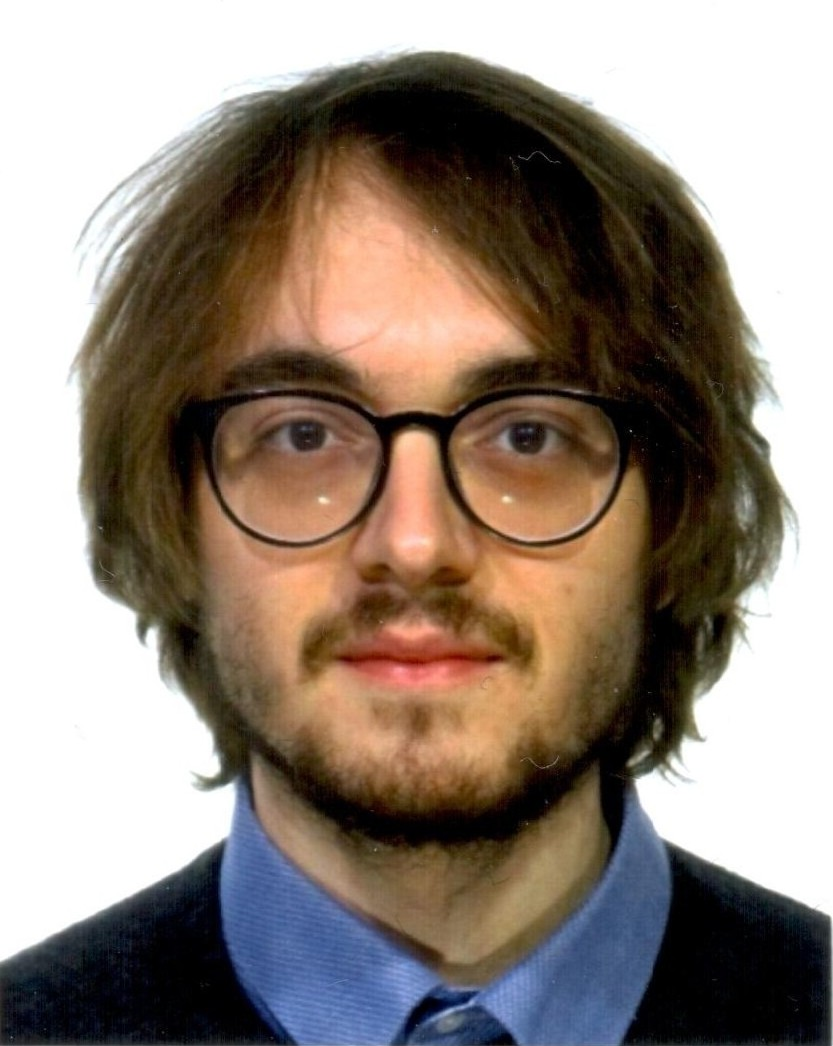
\includegraphics[width=0.65\textwidth]{Fototessera.jpg}\hfill\null

\vspace*{0.5ex} % Extra space after the picture

\headleft{Profile Summary}
Physics Master’s student specializing in Particles and Astroparticles with 2+ years of R\&D experience and active involvement in the JUNO international collaboration. Proven expertise in developing C++ (CERN ROOT) and Python data analysis tools for detector characterization and cosmogenic background reduction. Having worked in both fast-paced startups and large-scale collaborations, I am highly motivated to provide dedicated technical support to CERN’s large-scale projects.

\headleft{Contacts}
\small % To fit more content
\MVAt\ {\small nicolo.favagrossa@gmail.com} \\[0.4ex]
\Mobilefone\ +39\,389\,0155686 \\[0.5ex]
\faLinkedin\ \href{https://www.linkedin.com/in/nicolo-favagrossa/}{Nicolò Favagrossa}
\normalsize

\headleft{Personal Information}
Citizenship: \textbf{Italian} \\[0.5ex]
Languages: \\
\textbf{Italian} (Native) \\
\textbf{English C1} (University Certified)

\headleft{Soft Skills}
\begin{itemize}
\item Scientific Communication
\item Logico-Quantitative Analysis
\item Data Management \& Interpretation
\item High-Pressure Problem Solving
\item Autonomous Decision Making
\end{itemize}

\end{minipage}%
\kern0.09\textwidth\relax%%Right margin provided explicitly to stretch the colourbox
}
\end{minipage}% Right column
\hskip2.5em% Left margin for the white area
\begin{minipage}[t]{0.56\textwidth}
\setlength{\parskip}{0.8ex}% Adds spaces between paragraphs; use \\ to add new lines without this space. Shrink this amount to fit more data vertically

\vspace{2ex}

\headright{Professional Experience}

\textsc{Junior R\&D Lab Technician} | \textit{Prometheus S.p.A.} \textit{(Promoted from Assistant R\&D Technician in Jan 2025)} \dates{Nov 2023 – Present} \\
\smaller{Joined an early-stage energy startup, supporting its transition from a small laboratory to a large-scale R\&D facility at Kilometro Rosso.} \\
\smaller{Proposed and implemented original experimental campaigns and data acquisition strategies based on theoretical insights.} \\
\smaller{Developed numerical models using Python and C++ to validate physical phenomena; performed extensive scientific literature reviews to redesign experimental setups; calibrated complex sensors for high-precision measurement campaigns.}\\
\smaller{Acted as a technical bridge between internal R\&D, academic partners, and investors, delivering high-level scientific reports.}\\
\smaller{Collaborated within a heterogeneous and multidisciplinary team, assisting Senior Nuclear Engineers in the setup and operation of specialized nuclear instrumentation; developed practical hardware problem-solving skills in high-pressure laboratory environments.}

\headright{Education}

\textsc{Master's Degree in Physics} \\
\textit{Università degli Studi di Milano} \dates{2025 – Present} \\
\smaller{Specialization: Particle and astroparticle Physics.}

\is

\textsc{Bachelor’s Degree in Physics} \\
\textit{Università degli Studi di Milano} \dates{2020 – 2024} \\
\textit{Final Grade: 105/110 (GPA details included in academic transcript).}\\
\smaller{Thesis Title: Cosmic Muons in JUNO: Data Analysis of the Detector Filling Phase}

\headright{Research Experience}
\textsc{Undergraduate Researcher (Bachelor Thesis)} | \textit{JUNO International Collaboration} \dates{2024} \\
\smaller{Characterized the cosmic muon flux for the Jiangmen Underground Neutrino Observatory (JUNO) during the finale detector filling phase.}\\
\smaller{Developed an independent C++ (CERN ROOT) data analysis method to identify cosmic muon events from raw data; performed comparative benchmarking against official JUNO collaboration algorithms to validate event selection efficiency and detector response.}\\
\smaller{Successfully measured muon rates (compatible with the Monte Carlo expectation) and contributing to the optimization of detector veto strategies, essential for future solar neutrino measurements and cosmogenic background reduction.}\\

\headright{Technical and Others Skills}

\smaller{\textbf{Programming:} C++ (CERN ROOT, Simulations), Python (Modelling, Data Analysis), Linux (Bash, Terminal), Git/GitHub.} \\
\smaller{\textbf{Tools:} LaTeX (Scientific Documentation), Microsoft Office (Advanced Excel), Data Acquisition Software.} \\
\smaller{\textbf{Laboratory:} Nuclear Instrumentation, Sensor Calibration, Proactive Bibliographic Research.}

\end{minipage}

\end{document}
